% HS Vorlage
% ------------------------------------------------------------------------------
%   erstellt von Jannik Fangmann, 08.02.2013   
 
\documentclass[
    11pt, % Schriftgröße
    DIV10,
    ngerman, % für Umlaute, Silbentrennung etc.
    a4paper, % Papierformat
    oneside, % einseitiges Dokument
    titlepage, % es wird eine Titelseite verwendet
    parskip=half, % Abstand zwischen Absätzen (halbe Zeile)
    headings=normal, % Größe der Überschriften verkleinern
    listof=totoc, % Verzeichnisse im Inhaltsverzeichnis aufführen
    bibliography=totoc, % Literaturverzeichnis im Inhaltsverzeichnis aufführen
    index=totoc, % Index im Inhaltsverzeichnis aufführen
    captions=tableheading, % Beschriftung von Tabellen unterhalb ausgeben
    final % Status des Dokuments (final/draft)
]{scrartcl}

% Meta-Informationen -----------------------------------------------------------
%   Informationen über das Dokument, wie z.B. Titel, Autor, Matrikelnr. etc
%   werden in der Datei Meta.tex definiert und können danach global
%   verwendet werden.
% ------------------------------------------------------------------------------
% Meta-Informationen -----------------------------------------------------------
%   Definition von globalen Parametern, die im gesamten Dokument verwendet
%   werden können (z.B auf dem Deckblatt etc.).
%
%   ACHTUNG: Wenn die Texte Umlaute oder ein Esszet enthalten, muss der folgende
%            Befehl bereits an dieser Stelle aktiviert werden:
            \usepackage[utf8x]{inputenc}
% ------------------------------------------------------------------------------
\newcommand{\titel}{Essay im Bereich der Produktionslogistik}
\newcommand{\untertitel}{Möglichkeiten und Grenzen selbststeuernder produktionslogistischer Prozesse am Beispiel der Fertigung und Montage eines PKW-Rücklichtes}
\newcommand{\art}{PTP}
\newcommand{\modul}{Modul}
\newcommand{\themenstellung}{}
\newcommand{\autorA}{Jannik Fangmann}
\newcommand{\autorB}{Andreas Makeev}
\newcommand{\autorC}{Raphael Otten}
\newcommand{\autorD}{Carsten Sandker}
\newcommand{\studienbereich}{Wirtschaftsinformatik}
\newcommand{\matrikelnrA}{506347}
\newcommand{\matrikelnrB}{517007}
\newcommand{\matrikelnrC}{516975}
\newcommand{\matrikelnrD}{500199}
\newcommand{\semester}{Semester 6}
\newcommand{\gutachter}{Prof. Dr.-Ing. Marcus Seifert}
\newcommand{\abgabedatum}{\today}
\newcommand{\jahr}{2014}
\newcommand{\ort}{Lingen}
\newcommand{\logo}{HS_Osna_MKT.jpg}


% Erstellung eines Index aktivieren --------------------------------------------
\makeindex

% Anpassung des Seitenlayouts --------------------------------------------------
%   siehe Seitenstil.tex
% ------------------------------------------------------------------------------
\usepackage[
    automark, % Kapitelangaben in Kopfzeile automatisch erstellen
    headsepline, % Trennlinie unter Kopfzeile
    ilines % Trennlinie linksb�ndig ausrichten
]{scrpage2}

% Anpassung an Landessprache ---------------------------------------------------
\usepackage[ngerman]{babel}

% Umlaute ----------------------------------------------------------------------
%   Umlaute/Sonderzeichen wie äüöß direkt im Quelltext verwenden (CodePage).
%   Erlaubt automatische Trennung von Worten mit Umlauten.
% ------------------------------------------------------------------------------
\usepackage[utf8x]{inputenc}
\usepackage[T1]{fontenc}
\usepackage{textcomp} % Euro-Zeichen etc.

% Schrift ----------------------------------------------------------------------
\usepackage{lmodern} % bessere Fonts
\usepackage{relsize} % Schriftgröße relativ festlegen

% Grafiken ---------------------------------------------------------------------
% Einbinden von JPG-Grafiken ermöglichen
\usepackage[dvips,final]{graphicx}
% hier liegen die Bilder des Dokuments
\graphicspath{{Bilder/}}
  
% Befehle aus AMSTeX für mathematische Symbole z.B. \boldsymbol \mathbb --------
\usepackage{amsmath,amsfonts}

% für Index-Ausgabe mit \printindex --------------------------------------------
\usepackage{makeidx}

% Einfache Definition der Zeilenabst�nde und Seitenr�nder etc. -----------------
\usepackage{setspace}
\usepackage{geometry}

% Symbolverzeichnis ------------------------------------------------------------
%   Symbolverzeichnisse bequem erstellen. Beruht auf MakeIndex:
%     makeindex.exe %Name%.nlo -s nomencl.ist -o %Name%.nls
%   erzeugt dann das Verzeichnis. Dieser Befehl kann z.B. im TeXnicCenter
%   als Postprozessor eingetragen werden, damit er nicht ständig manuell
%   ausgeführt werden muss.
%   Die Definitionen sind ausgegliedert in die Datei "Glossar.tex".
% ------------------------------------------------------------------------------
\usepackage[intoc]{nomencl}
\let\abbrev\nomenclature
\renewcommand{\nomname}{Abkürzungsverzeichnis}
\setlength{\nomlabelwidth}{.25\hsize}
\renewcommand{\nomlabel}[1]{#1 \dotfill}
\setlength{\nomitemsep}{-\parsep}

% zum Umfließen von Bildern ----------------------------------------------------
\usepackage{floatflt}
\usepackage{float}

% zum Einbinden von PDFs ------------------------------------------------------
\usepackage{pdfpages}

% zum Einbinden von Programmcode -----------------------------------------------
\usepackage{listings}
% Einstellungen zum listings-Package
\lstset{
    float=hbp,
    basicstyle=\footnotesize,
    columns=flexible,
    tabsize=2,
    frame=single,
    extendedchars=true,
    showspaces=false,
    showstringspaces=false,
    numbers=left,
    numberstyle=\tiny,
    breaklines=true,
    breakautoindent=true,
    captionpos=b,
    }
\usepackage{xcolor} 
\definecolor{hellgelb}{rgb}{1,1,0.9}
\definecolor{colKeys}{rgb}{0,0,1}
\definecolor{colIdentifier}{rgb}{0,0,0}
\definecolor{colComments}{rgb}{0,0.5,0}
\definecolor{colString}{rgb}{1,0,0}
\lstset{
    float=hbp,
    basicstyle=\ttfamily\color{black}\small\smaller,
    identifierstyle=\color{colIdentifier},
    keywordstyle=\color{colKeys},
    stringstyle=\color{colString},
    commentstyle=\color{colComments},
    columns=flexible,
    tabsize=2,
    frame=single,
    extendedchars=true,
    showspaces=false,
    showstringspaces=false,
    numbers=left,
    numberstyle=\tiny,
    breaklines=true,
    backgroundcolor=\color{hellgelb},
    breakautoindent=true
}
% http://blog.yeticode.co.uk/2009/04/c-sharp-style-for-lstinputlisting/
\lstdefinelanguage{cs}
  {morekeywords={abstract,event,new,struct,as,explicit,null,switch
		base,extern,object,this,bool,false,operator,throw,
		break,finally,out,true,byte,fixed,override,try,
		case,float,params,typeof,catch,for,private,uint,
		char,foreach,protected,ulong,checked,goto,public,unchecked,
		class,if,readonly,unsafe,const,implicit,ref,ushort,
		continue,in,return,using,decimal,int,sbyte,virtual,
		default,interface,sealed,volatile,delegate,internal,short,void,
		do,is,sizeof,while,double,lock,stackalloc,
		else,long,static,enum,namespace,string, },
	  sensitive=false,
	  morecomment=[l]{//},
	  morecomment=[s]{/*}{*/},
	  morestring=[b]",
}
\lstdefinelanguage{natural}
  {morekeywords={DEFINE,DATA,LOCAL,END-DEFINE,WRITE,CALLNAT,PARAMETER,USING,%
               IF,NOT,END-IF,ON,*ERROR-NR,ERROR,END-ERROR,ESCAPE,ROUTINE,%
               PERFORM,SUBROUTINE,END-SUBROUTINE,CONST,END-FOR,END,FOR,RESIZE,%
               ARRAY,TO,BY,VALUE,RESET,COMPRESS,INTO,EQ},
	  sensitive=false,
	  morecomment=[l]{/*},
	  morestring=[b]",
	  morestring=[b]',
	  alsodigit={-,*},
}


% URL verlinken, lange URLs umbrechen etc. -------------------------------------
\usepackage{url}

% wichtig für korrekte Zitierweise ---------------------------------------------
\usepackage[square]{natbib}

% PDF-Optionen -----------------------------------------------------------------
\usepackage[
    bookmarks,
    bookmarksnumbered,    
    bookmarksopen=true,
    bookmarksopenlevel=1,
    colorlinks=true,
% diese Farbdefinitionen zeichnen Links im PDF farblich aus
    %linkcolor=red, % einfache interne Verkn�pfungen
    %anchorcolor=black,% Ankertext
    %citecolor=blue, % Verweise auf Literaturverzeichniseintr�ge im Text
    %filecolor=magenta, % Verkn�pfungen, die lokale Dateien �ffnen
    %menucolor=red, % Acrobat-Men�punkte
    %urlcolor=cyan, 
% diese Farbdefinitionen sollten f�r den Druck verwendet werden (alles schwarz)
    linkcolor=black, % einfache interne Verkn�pfungen
    anchorcolor=black, % Ankertext
    citecolor=black, % Verweise auf Literaturverzeichniseintr�ge im Text
    filecolor=black, % Verkn�pfungen, die lokale Dateien �ffnen
    menucolor=black, % Acrobat-Men�punkte
    urlcolor=black, 
%
    backref,
    pdftex,
    plainpages=false, % zur korrekten Erstellung der Bookmarks
    pdfpagelabels=true, % zur korrekten Erstellung der Bookmarks
    hypertexnames=true, % zur korrekten Erstellung der Bookmarks
    linktocpage % Seitenzahlen anstatt Text im Inhaltsverzeichnis verlinken
]{hyperref}
% Befehle, die Umlaute ausgeben, f�hren zu Fehlern, wenn sie hyperref als Optionen �bergeben werden
\hypersetup{
    pdftitle={\titel \untertitel},
    pdfauthor={\autorA},
    pdfcreator={\autorA},
    pdfsubject={\titel \untertitel},
    pdfkeywords={\titel \untertitel},
}

% fortlaufendes Durchnummerieren der Fu�noten ----------------------------------
\usepackage{chngcntr}

% für lange Tabellen -----------------------------------------------------------
\usepackage{longtable}
\usepackage{array}
\usepackage{ragged2e}
\usepackage{lscape}

% Spaltendefinition rechtsb�ndig mit definierter Breite ------------------------
\newcolumntype{w}[1]{>{\raggedleft\hspace{0pt}}p{#1}}

% Formatierung von Listen �ndern -----------------------------------------------
\usepackage{paralist}

% bei der Definition eigener Befehle benötigt
\usepackage{ifthen}

% definiert u.a. die Befehle \todo und \listoftodos
\usepackage{todonotes}

% sorgt dafür, dass Leerzeichen hinter parameterlosen Makros nicht als
% Makroendezeichen interpretiert werden
\usepackage{xspace}

% Erstellen von Struktogrammen (Nassi-Shneidermann)
\usepackage{struktex}

% Durchstreichen von Text
\usepackage{cancel}

% Packages zur Gestaltung von Tabellen
\usepackage{color}
\usepackage{colortbl}
\usepackage{tabularx} 
\usepackage{multicol} 
\usepackage{multirow} 
\usepackage{booktabs}

% Farben für Tabellen
\definecolor{dunkelgrau}{rgb}{0.8,0.8,0.8}
\definecolor{hellgrau}{rgb}{0.95,0.95,0.95}



% Kopf- und Fußzeilen, Seitenränder etc. ---------------------------------------
% Zeilenabstand 1,5 Zeilen -----------------------------------------------------
\onehalfspacing

% Überschriften (Chapter höher setzen)
\renewcommand*{\chapterheadstartvskip}{\vspace*{-\topskip}}

% Seitenränder -----------------------------------------------------------------
\setlength{\topskip}{\ht\strutbox} % behebt Warnung von geometry
\geometry{paper=a4paper,left=20mm,right=40mm,top=20mm,bottom=45mm}

% Kopf- und Fußzeilen ----------------------------------------------------------
\pagestyle{scrheadings}
% Kopf- und Fußzeile auch auf Kapitelanfangsseiten
%\renewcommand*{\chapterpagestyle}{scrheadings} 
% Schriftform der Kopfzeile
\renewcommand{\headfont}{\normalfont}

% Kopfzeile
\ihead{\large{\textsc{\titel}}\\ \small{\untertitel} \\[2ex]
\textit{\headmark}}
\chead{}
\ohead{\includegraphics[scale=0.5]{\logo}}
\setlength{\headheight}{21mm} % Höhe der Kopfzeile
% Kopfzeile über den Text hinaus verbreitern
\setheadwidth[0pt]{textwithmarginpar} 
\setheadsepline[text]{0.4pt} % Trennlinie unter Kopfzeile

% Fußzeile
\ifoot{\copyright \ \autorA}
\cfoot{}
\ofoot{\pagemark}

% Größe der Fußzeilenschriftgröße auf 9pt anpassen
\def\footnotesize{\fontsize{9pt}{10pt}\selectfont}

% sonstige typographische Einstellungen ----------------------------------------

% erzeugt ein wenig mehr Platz hinter einem Punkt
\frenchspacing 

% Schusterjungen und Hurenkinder vermeiden
\clubpenalty = 10000
\widowpenalty = 10000 
\displaywidowpenalty = 10000

% Quellcode-Ausgabe formatieren
\lstset{numbers=left, numberstyle=\tiny, numbersep=5pt, breaklines=true}
\lstset{emph={square}, emphstyle=\color{red}, emph={[2]root,base}, emphstyle={[2]\color{blue}}}

% Fu�noten fortlaufend durchnummerieren
%\counterwithout{footnote}{chapter}


% eigene LaTeX-Befehle
% Eigene Befehle und typographische Auszeichnungen f�r diese

% einfaches Wechseln der Schrift, z.B.: \changefont{cmss}{sbc}{n}
\newcommand{\changefont}[3]{\fontfamily{#1} \fontseries{#2} \fontshape{#3} \selectfont}

% Abk�rzungen mit korrektem Leerraum 
\newcommand{\ca}{ca.\ }
\newcommand{\Vgl}{Vgl.\ }
\newcommand{\bzw}{bzw.\ }
\newcommand{\etc}{etc.\ }
\newcommand{\inkl}{inkl.\ }
\newcommand{\evtl}{evtl.\ }
\newcommand{\ggfs}{ggfs.\ }
\newcommand{\usw}{usw.\ }

\newcommand{\abbildung}[1]{Abbildung~\ref{fig:#1} (\nameref{fig:#1})}
\newcommand{\listing}[1]{Listing~\ref{lst:#1} (\nameref{lst:#1})}
\newcommand{\verweis}[1]{Abschnitt~\ref{sec:#1} (\nameref{sec:#1})}

\newcommand{\bs}{$\backslash$}

\newcommand{\AO}{\textsc{Alte Oldenburger}\xspace}

% Setzt ein Wort in Anführungszeichen
\newcommand{\gqq}[1]{\glqq{}#1\grqq{}}

% erzeugt ein Listenelement mit fetter Überschrift 
\newcommand{\itemd}[2]{\item{\textbf{#1}}\\{#2}}

% einige Befehle zum Zitieren --------------------------------------------------
\newcommand{\Zitat}[2][\empty]{\ifthenelse{\equal{#1}{\empty}}{\citep{#2}}{\citep[#1]{#2}}}

% zum Ausgeben von Autoren
\newcommand{\Autor}[1]{\textsc{#1}}

% verschiedene Befehle um Wörter semantisch auszuzeichnen ----------------------
\newcommand{\Index}[2][\empty]{\ifthenelse{\equal{#1}{\empty}}{\index{#2}#2}{\index{#1}#2}}
\newcommand{\Fachbegriff}[2][\empty]{\ifthenelse{\equal{#1}{\empty}}{\textit{\Index{#2}}}{\textit{\Index[#1]{#2}}}}
\newcommand{\NeuerBegriff}[2][\empty]{\ifthenelse{\equal{#1}{\empty}}{\textbf{\Index{#2}}}{\textbf{\Index[#1]{#2}}}}

\newcommand{\Ausgabe}[1]{\texttt{#1}}
\newcommand{\Eingabe}[1]{\texttt{#1}}
\newcommand{\Code}[1]{\texttt{#1}}
\newcommand{\Datei}[1]{\texttt{#1}}

\newcommand{\Assembly}[1]{\textsf{#1}}
\newcommand{\Klasse}[1]{\textsf{#1}}
\newcommand{\Methode}[1]{\textsf{#1}}
\newcommand{\Attribut}[1]{\textsf{#1}}

\newcommand{\Datentyp}[1]{\textsf{#1}}
\newcommand{\XMLElement}[1]{\textsf{#1}}
\newcommand{\Webservice}[1]{\textsf{#1}}

\newcommand{\Refactoring}[1]{\Fachbegriff{#1}}
\newcommand{\CodeSmell}[1]{\Fachbegriff{#1}}
\newcommand{\Metrik}[1]{\Fachbegriff{#1}}
\newcommand{\DesignPattern}[1]{\Fachbegriff{#1}}


% Das eigentliche Dokument -----------------------------------------------------
%   Der eigentliche Inhalt des Dokuments beginnt hier. Die einzelnen Seiten
%   und Kapitel werden in eigene Dateien ausgelagert und hier nur inkludiert.
% ------------------------------------------------------------------------------
\begin{document}

% auch subsubsection nummerieren
\setcounter{secnumdepth}{3}
\setcounter{tocdepth}{3}

% Deckblatt und Abstract ohne Seitenzahl
\ofoot{}
\thispagestyle{plain}
\begin{titlepage}

\begin{center}

\Huge{\textbf{\titel}}\\[1.4ex]
\huge{mit der Themenstellung:\\ {\untertitel}}\\[6ex]


\includegraphics[scale=1.2]{HS_Osna_MKT.jpg}\\[7ex]

\normalsize
\begin{tabular}{w{5.4cm}p{6cm}}\\
vorgelegt von:  & \quad \autorA \quad (\matrikelnrA)\\[1.2ex]
        & \quad \autorB \quad (\matrikelnrB)\\[1.2ex]
        & \quad \autorC \quad (\matrikelnrC)\\[1.2ex]
        & \quad \autorD \quad (\matrikelnrD)\\[1.2ex]
Studienbereich: & \quad \studienbereich\\[1.2ex]
Semester: & \quad \semester\\[1.2ex]
Gutachter:  & \quad \gutachter\\[1.2ex]
Abgabedatum: & \quad \abgabedatum\\[2.4ex]
\end{tabular}

\copyright\ \jahr\\[12ex]

\end{center}

\singlespacing
\small
\noindent Dieses Werk einschließlich seiner Teile ist \textbf{urheberrechtlich
geschützt}. Jede Verwertung außerhalb der engen Grenzen des Urheberrechtgesetzes
ist ohne Zustimmung des Autors unzulässig und strafbar. Das gilt insbesondere
für Vervielfältigungen, Übersetzungen, Mikroverfilmungen sowie die
Einspeicherung und Verarbeitung in elektronischen Systemen.

\end{titlepage}


% Abstract----------------------------------------------------------------------
% \include{Inhalt/Abstract}
% ------------------------------------------------------------------------------
\ofoot{\pagemark}

% Seitennummerierung -----------------------------------------------------------
%   Vor dem Hauptteil werden die Seiten in gro�en r�mischen Ziffern 
%   nummeriert.
% ------------------------------------------------------------------------------

\pagenumbering{Roman}
\pdfbookmark[1]{Inhaltsverzeichnis}{toc} % Inhaltsverzeichnis als PDF-Bookmark
\tableofcontents % Inhaltsverzeichnis

% Abk�rzungsverzeichnis --------------------------------------------------------
% \input{Inhalt/Glossar}

% für korrekte Überschrift in der Kopfzeile
% \clearpage
%\markboth{\nomname}{\nomname} 

% Abbildungsverzeichnis --------------------------------------------------------
% \listoffigures 
% ------------------------------------------------------------------------------

% arabische Seitenzahlen im Hauptteil ------------------------------------------
\clearpage
\pagenumbering{arabic}

% die Inhaltskapitel werden in "Inhalt.tex" inkludiert -------------------------
% Hier können die einzelnen Kapitel inkludiert werden. Sie müssen in den 
% entsprechenden .TEX-Dateien vorliegen. Die Dateinamen können natürlich 
% angepasst werden.

\section{Einleitung}
\label{sec:Einleitung}
Heutzutage wünschen sich Kunden immer mehr Produkte ihren eigenen Vorstellungen
anzupassen und individuell gestalten zu können. Um diesen Kundenwünschen gerecht
zu werden, ist es notwendig sich als Unternehmen diesen dynamischen Änderungen
anzupassen.  Der Bekleidunghersteller Nike sowie der Autohersteller Opel haben
diese Entwicklung erkannt und bieten ihren Kunden bei bestimmten Produktmodellen
die Möglichkeit zur Individualisierung.\footnote{Nike Konfigurator NIKEiD:
\url{http://www.nike.com/de/de_de/c/nikeid/}} So bietet Opel zum Beispiel bei
seinem Automodell „Adam“ die individuelle Konfiguration nach speziellen
Kundenwünschen an.\footnote{Opel Adam Konfigurator:
\url{http://konfigurator.opel-adam.de/}} Dort ist es möglich das Auto in den
Bereichen Motor, Außen- und Innendesign, Sonderausstattung, etc. zu
konfigurieren und in dieser individuellen Konfiguration zu bestellen. Aus der
so entstehenden Variantenvielfalt der Produkte resultiert eine gesteigerte
Komplexität im Produktionsprozess.

Ein Ansatz, die Flexibilität trotz der gestiegener Komplexität zu gewährleisten,
ist die Einführung selbststeuernder Prozesse. Dieser Ansatz wurde in dem
Sonderforschungsbereich 637 der Universität Bremen in einem Forschungsprojekt
thematisiert. In dem Projekt wurde die Selbststeuerung von Prozessen am Beispiel
des Produktionsprozesses von PKW-Rücklichtern näher untersucht. An diesem Punkt
setzt diese Arbeit an und beschreibt die Möglichkeiten der selbststeuernden
Prozesse anhand dieses Fallbeispiels.

Ziel ist es den Prozess aus dem Fallbeispiel mit der Realisierung in einem
klassischen Fließfertigungsprozess zu vergleichen, um Möglichkeiten und Grenzen
von selbststeuernden Prozessen im Vergleich zur Fließfertigung zu
identifizieren.

Um zunächst ein einheitliches Verständnis in diesem Bereich zu schaffen, wird
die Definition des selbststeuernden Prozesses erläutert. Aufbauend auf der
theoretischen Definition wird das bereits erwähnte Forschungsbeispiel der
Universität Bremen aufgegriffen und näher betrachtet. Anhand des Beispiels
werden zunächst die Möglichkeiten der selbststeuernden Prozesse in der
Produktionslogistik aufgezeigt. Im Nachhinein wird ein klassischer Prozess
modelliert, mit dem der selbststeuernde Prozess verglichen wird, um Vorteile
beider Prozesse aufzuzeigen. Hierauf aufbauend werden die Grenzen von
selbststeuernden Prozessen erläutert. Zum Schluss werden in einem abschließenden
Fazit die gewonnenen Erkenntnisse in dieser Ausarbeitung reflektiert.

\clearpage
%ToDo: Link auf Nike noch anpassen
\section{Definition}
\label{sec:Definition}

\begin{quote}
“Selbststeuerung beschreibt Prozesse dezentraler Entscheidungsfindung in heterarchischen Strukturen. 
Sie setzt voraus, dass interagierende Elemente in nichtdeterministischen Systemen die Fähigkeit und 
Möglichkeit zum autonomen Treffen von Entscheidungen besitzen.”\footnote{XX}
\end{quote}

Diese Definition der selbststeuernden Prozesse sagt aus, dass ein zentrales Merkmal der Selbststeuerung 
ist, dass die einzelnen Elemente im Produktionsprozess selbstständig Entscheidungen fällen können. 
Dieser eigenständige Entscheidungsprozess kann dadurch ermöglicht werden, dass der gesamte Prozess 
eine nicht hierarchische Struktur besitzt und jedes Element damit selbst entscheidungsberechtigt ist. 
Dadurch wird eine Dezentralisierung des Entscheidungsprozesses vom Gesamtsystem auf die einzelnen 
Systemelemente generiert. Die Entscheidungen jedes einzelnen Systemelements basieren dabei auf Informationen 
und Eigenschaften, die jedes Element besitzt. Anhand dieser wird, bei Eintreten eines nicht geplanten 
Systemzustandes des Gesamtsystems, eine Entscheidung  gefällt. Der Eintritt von nicht geplanten Zuständen 
des Gesamtsystems ist dabei der nicht-deterministischen Eigenschaft geschuldet.
"`Unter Nicht-Determinismus wird verstanden, dass trotz genauester Messung des Systemzustandes 
und der Kenntnis aller wirkenden Systemgesetze keine Vorhersage des Systemverhaltens über einen längeren Zeitraum 
möglich ist."'\footnote{\citet[S.~15]{boese2012}}
\section{Forschungsbeispiel}
\label{sec:Forschungsbeispiel}

Im Rahmen dieser Ausarbeitung sollen die Möglichkeiten und Grenzen selbststeuernder 
Prozesse in der Produktionslogistik untersucht werden. Die Untersuchung soll hierbei 
anhand eines Forschungsprojektes des Sonderforschungsbereichs 637 „Selbststeuerung 
logistischer Prozesse – Ein Paradigmenwechsel und seine Grenzen“ der Universität 
Bremen durchgeführt werden. Der Sonderforschungsbereich befasst sich mit der Frage, 
auf welche Weise sich Modelle, Methoden und Werkzeuge logistischer Prozesse abändern 
lassen, um eine dezentrale Selbststeuerung zu ermöglichen.

Bei dem zu untersuchenden Forschungsprojekt handelt es sich um eine Demonstrationsplattform, 
die die vom Sonderforschungsbereich erarbeiteten Selbststeuerungskonzepte anschaulich 
darstellen soll. Die Demonstrationsplattform bildet ein Produktionsszenario für die Montage 
von PKW-Rücklichtern ab. Der Montageprozess ermöglicht hierbei die Fertigung verschiedener 
Produktvarianten der PKW-Rücklichter. Weiterhin können innerhalb des Montageprozesses verschiedene 
Montagestationen flexibel durchlaufen werden. In den Produktionsprozess sind hierbei verschiedene 
Methoden der Selbststeuerung implementiert. \abbildung{Montagestation} zeigt die einzelnen Montagestationen der Demonstrationsplattform.

\begin{figure}[htb] 
\centering
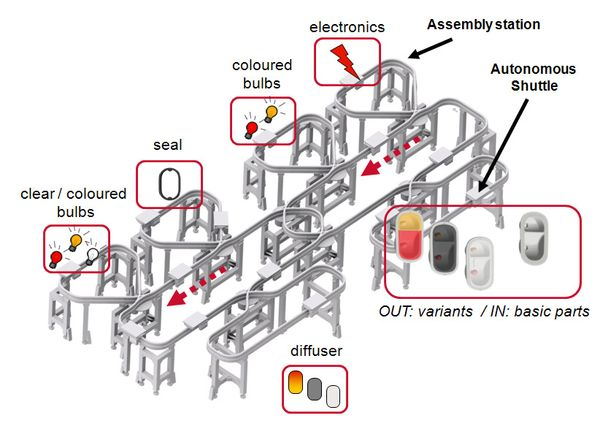
\includegraphics[width=1.0\textwidth]{Montage.jpg}
\caption[Montagestation]{Montagestationen der Demonstrationsplattform\protect\footnotemark}
\label{fig:Montagestation}
\end{figure}
\footnotetext{entnommen aus \citet[S.~xx]{xx}}

Die Demonstrationsplattform besteht aus einem Einschienensystem, auf dem sich mehrere 
Transportplattformen, sogenannte Shuttle, autonom bewegen können. Die Shuttle transportieren 
die Rücklichter einzeln durch das Montagesystem. Zu Beginn des Montageprozesses wird ein 
Reflektor-Gussteil, welcher das Ausgangsbauteil der Montage darstellt, auf dem Shuttle 
angebracht. In jedes dieser Reflektor-Gussteil wurde dabei ein RFID-Transponder integriert, 
welcher die Eindeutige Identifikation des Bauteils über den gesamten Montageprozess hinweg ermöglicht.
Im Verlauf des Montageprozesses wird das Ausgangsbauteil an verschiedenen Montagestationen um die 
Komponenten Kabelbaum, Leuchtmittel, Dichtung und Blende erweitert. Die Reihenfolge, in der die 
einzelnen Komponenten an den Reflektor angebracht werden können, ist dabei flexibel. Es müssen 
jedoch bestimmte Abhängigkeiten eingehalten werden. So müssen beispielsweise Leuchtmittel und 
Dichtung vor der Blende montiert werden. Der Kabelbaum kann hingegen zu jeder Zeit an dem Reflektor angebracht werden.

\begin{figure}[htb] 
\centering
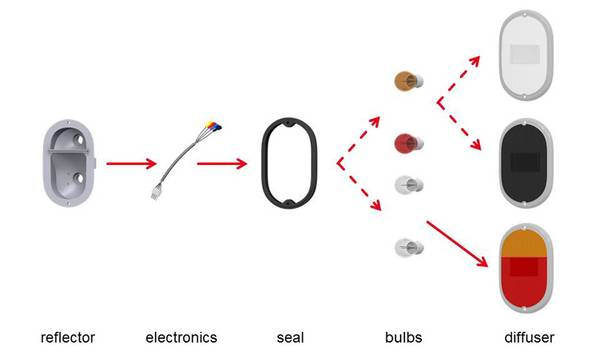
\includegraphics[width=1.0\textwidth]{Variantenkorridor.jpg}
\caption[Variantenkorridor]{Variantenkorridor\protect\footnotemark}
\label{fig:Variantenkorridor}
\end{figure}
\footnotetext{entnommen aus \citet[S.~xx]{XX}}


\subsection{Erkennbare Möglichkeiten von selbststeuernden Prozessen im Beispiel}
\label{sec:Moeglichkeiten}

Die innerhalb des Beispiels erkannten Möglichkeiten im Bezug auf die Fertigung
von PKW-Rücklichtern, werden nun konkret betrachtet. Hierbei werden
unterschiedliche Sichtweisen der Betrachtung angewendet. So gibt es die
Auftragssicht und die Ressourcensicht.\footnote{\citet[S.~234]{arnold2008}}
Die Auftragssicht beschreibt dabei die Struktur eines Auftrages und dessen Durchlauf in der Wertschöpfungskette. Die
Ressourcensicht bildet hingegen den Materialfluss innerhalb der Produktion ab.
Unter Beachtung dieser beiden Sichten ergeben sich folgende Möglichkeiten aus
dem vorher dargestellten Beispiel:

\paragraph{Schnelle Reaktion auf sich ändernde Kundenwünsche /
Marktsituationen} \hfill \\
Im Beispiel ist es möglich sehr schnell auf sich ändernde Kundenwünsche oder
Marktsituationen innerhalb der Produktion zu reagieren. Sollte der Absatz einer
Produktvariante oder die Bestellung eines Kunden sich zur Laufzeit der Montage
ändern, kann auf diese neue Situation sofort reagiert werden. Durch die bereits
erwähnten RFID-Chips in den Produkten können die Softwareagenten die Produkte
innerhalb der Produktion reorganisieren. Dies bedeutet, dass alle Produkte
angepasst an den neuen Auftrag gefertigt werden. Konkret werden halbfertige
Produkte vom stornierten Auftrag übernommen und mit den gewünschten neuen
Parametern des aktuellen Auftrags fertiggestellt. Die Abhängigkeiten des
vorgestellten Variantenkorridors sind hierbei zu beachten. So könnten Produkte,
die bereits mit weißen Leuchtmitteln ausgestattet sind, nicht mehr mit einer
durchsichtigen oder schwarzen Blende versehen werden. Wenn im aktuellen Auftrag
keine PKW-Rücklichter mit weißen Leuchtmitteln gefordert sind, entsteht in
diesem Fall eine kleine Menge an Ausschussware. Diese könnte in einem
nachfolgenden Auftrag aber weiter verarbeitet werden.

\paragraph{Lastverteilung} \hfill \\
Innerhalb des Beispiels ist eine Lastverteilung unter den einzelnen
Bearbeitungstationen möglich. Ist beispielsweise die Bearbeitungsstation der
Kabelbauminstallation besetzt, entsteht keine Wartezeit für ein anderes Produkt.
Dieses wird unter Beachtung des Variantenkorridors an einer anderen freie
Arbeitsstation weitergeleitet, d.h. es wird beispielsweise zuerst das
Leuchtmittel oder die Dichtung montiert, bevor der Kabelbaum verlegt wird.
Denkbar wäre es auch, dass somit die unterschiedlichen Bearbeitungszeiten der
Stationen ausgeglichen werden.
%TODO: Punkt wird zu kurz Angesprochen??

\paragraph{Vermeidung von Stillstandszeiten}\hfill \\
Sollte in dem dargestellten Beispiel eine Station kurzfristig ausfallen, so
leiten sich Produkte selbstständig auf eine alternative Station um. Hierbei 
werden, genau wie bei der Lastverteilung, die Abhängigkeiten aus dem
Variantenkorridor beachtet. Die gesamte Produktion würde, mit Ausnahme der
ausgefallenen Arbeitsstation, weitergeführt werden. Während andere
Montageschritte weiterhin durchlaufen werden, wird die Montagestation instand
gesetzt. Sobald der Fehler behoben ist, kann die Station wieder in Betrieb
genommen werden. Diese gliedert sich daraufhin automatisch in den Arbeitsablauf
ein und kann von den Bauteilen erneut durchlaufen werden.

\paragraph{Fertigung von mehreren Varianten zur Laufzeit} \hfill \\
Mit dem vorgestellten Beispielprozess ist es möglich verschiedene Varianten des
PKW-Rücklichtes zeitgleich in einer Produktionsstraße zu produzieren. Die
Information, welche Module im Produkt verbaut werden, ist direkt an jedem
einzelnen Rücklicht gespeichert. Hierzu ist in jedem Rücklicht ein RFID-Chip
eingelassen. Die Informationen werden an den einzelnen Bearbeitungsstationen
eingelesen und der Maschine / dem Arbeiter angezeigt. Es wird so garantiert,
dass jedes Produkt der Bestellung entspricht. Hiermit ergibt sich die
Möglichkeit in dem Beispielprozess alle drei Varianten gleichzeitig
herzustellen. Denkbar wäre, dass sich das Rücklicht der Variante 1 innerhalb
der Lampenmontage befindet und das Rücklicht der Variante 2 zeitgleich in der
Blendenmontage.


\section{Grenzen selbststeuernder produktionslogistischer Prozesse}
\label{sec:Grenzen}

Im vorherigen Kapitel wurden die erarbeiteten Möglichkeiten der
selbststeuernden Prozesse aus dem Beispiel einem vergleichbaren Prozess der
Fließfertigung gegenübergestellt. Hieraus ergeben sich Vorteile von
selbststeuernden Prozessen. Im Folgenden wollen wir veranschaulichen,
das selbststeuernde Prozesse aber auch ihre Grenzen haben.

Die Grenzbetrachtung basiert auf der Darstellung aus \citet{evolution2007}.
In die dort beschriebene Grenzbetrachtung werden die beiden zuvor 
betrachteten Prozesse integriert und die Grenzen von selbsteuernden 
Prozessen werden daraus abgeleitet. Eine Darstellung dieser Grenzbetrachtung
mit der Einordnung des beschriebenen selbststeuernden und klassischen Prozesses
zeigt die folgende \abbildung{Grenzbetrachtung}:
 
\begin{figure}[htb] 
\centering
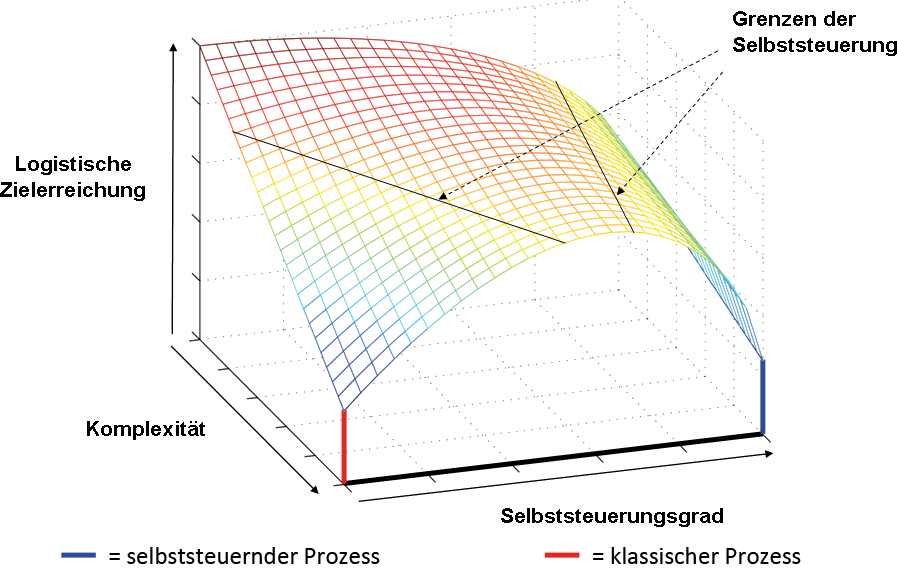
\includegraphics[width=1.0\textwidth]{Grenzbetrachtung.png}
\caption[Grenzbetrachtung]{Grenzen selbststeuernder Prozesse\protect\footnotemark}
\label{fig:Grenzbetrachtung}
\end{figure}
\footnotetext{in Anlehnung an \citet[S.~3]{evolution2007}}

Hierbei gilt es von Anfang an zu verdeutlichen, dass in der dargestellten
Grenzbetrachtung die Grenzen anhand einer "`logistischen Zielerreichung"'
festgelegt wurden. Diese logistische Zielerreichung setzt sich dabei zusammen
aus mehreren gewichteten produktionslogistischen Kennzahlen wie zum Beispiel
hohe Termintreue, mittlere Durchlaufzeiten, Bestände und Auslastung.\footnote{Vgl. \citet[S.~4]{evolution2007}}
Diese logistische Zielerreichung entspricht dabei nicht den Kriterien,
die für den vorherigen Vergleich herangezogen wurden. 

Aus der dargestellten Abbildung haben wir zwei Grenzen des selbststeuernden
Prozesses im Hinblick auf ihre logistische Zielerreichung herausgearbeitet.

Zunächst kann in der Abbildung gesehen werden, dass die logistische Zielerreichung
des selbststeuernden Prozesses bei der dargestellten Komplexität sehr gering ist.
Diese geringe Zielerreichung können wir mit dem Fehlen von zentralen 
Eingriffs- und Kontrollmöglichkeiten begründen. Dazu ist zu sehen, dass der
Selbststeuerungsgrad des selbststeuernden Prozess in der obigen Abbildung bei 100\% liegt. Aufgrund 
dieser vollständigen Autonomie kann auf eintretende Produktionsfehler nur mit zwei
Möglichkeiten reagiert werden:

\begin{enumerate}
  \item Maschine(n) neu programmieren (Zeitaufwand)
  \item Maschine(n) abschalten (Kostenaufwand)
\end{enumerate}

Beide Möglichkeiten sind dabei aus produktionslogistischer Sicht ungünstig.
Wir folgern daraus, dass Selbststeuerung immer zentrale Eingriffs- und Kontrollmöglichkeiten
benötigt und vollständige Produktionsautonomie nicht das Ziel sein kann. Dieser \textbf{Kontrollverlust
bei vollständiger Selbststeuerung} ist die erste Grenze selbststeuernder Prozesse
die wir erarbeiten konnten.

Der geringen Zielerreichung des selbststeuernden Prozesses steht ein relativ
hoher Grad der Zielerreichung beim klassischen Prozess gegenüber.
Diese Diskrepanz der Zielerreichung führen wir auf die geringe
Komplexität des betrachteten Produktionsprozesses zurück.
Der betrachtete Produktionsprozess der Rücklichterfertigung besteht nur aus
drei verschiedenen Varianten und vier Fertigungsmaschinen und ist aus diesem
Grund mit dargestellter geringer Komplexität eingeordnet. Diese geringe
Komplexität ermöglicht es, dass der klassische Prozesse effektiv über ein zentrales
System ohne Selbststeuerung gesteuert werden kann (in unserm Beispiel wäre dies der Produktionsplan).
Bei dieser geringen Komplexität fehlt der Bedarf nach Selbststeuerung bzw. autonomer Entscheidungsfindung,
da auch ohne diese die produktionslogistischen Ziele erreicht werden können.
Weiterhin spart man beim Einsatz eines klassischen Prozesses die Kosten für 
die Implementierung einer Selbststeuerung und es wird kein zusätzliches 
Know-How benötigt. Die Grenze die wir hier feststellen ist der \textbf{fehlende Mehrwert}
selbststeuernder Prozesse \textbf{bei geringer Komplexität}.
Diese Grenze können wir weiterhin begründen, wenn das Verhalten beider Prozesse
bei zunehmender Komplexität betrachtet wird.

Steigt die Komplexität in dargestellter \abbildung{Grenzbetrachtung} ist zu erkennen,
dass die logistische Zielerreichung des klassischen Prozesses signifikant abnimmt.
Eine zentrale Steuerung der Produktionsprozesse, z.B. in Form eines Produktionsplans,
kann die gestiegene Komplexität nicht mehr effektiv umsetzen. Mit zunehmender 
Selbststeuerung steigt dagegen die Zielerreichung bei maximaler Komplexität. Die 
zuvor erläuterten Vorteile der Selbststeuerung können in diesem Szenario effektiv
genutzt werden.

\clearpage
\paragraph{Fazit der Grenzbetrachtung}\mbox{}\\

In dieser Genzbetrachtung haben wir 2 Grenzen von selbststeuernden Prozessen
herausgearbeitet:

\begin{enumerate}
  \item Kontrollverlust bei vollständiger Selbststeuerung
  \item Fehlender Mehrwert bei geringer Komplexität
\end{enumerate}

Diese Grenzbetrachtung basiert dabei auf den dargestellten Indikatoren der logistischen
Zielerreichnug und nicht auf den Indikatoren die beim vorherigen Vergleich herangezogen wurden.

% Im Folgenden werden die in der Darstellung unterstellten Grenzen der
% Selbststeuerung untersucht. Die dargestellten Grenzen lassen sich dabei in drei
% Mängel unterscheiden, die bei bestimmten Produktionssituationen vorliegen:

% \begin{itemize}
%   \item Fehlender Mehrwert bei geringer Komplexität
%   \item Fehlender Mehrwert bei Make-to-Stock-Produkten
%   \item Kontrollverlust als Grenzen der Selbststeuerung
% \end{itemize}

% Die Unterscheidung in diese drei Grenzbereiche werden in den nachfolgenden 
% Abschnitten näher erläutert.

% \subsection{Fehlender Mehrwert bei geringer Komplexität}
\label{sec:GrenzenKomplexitaet}

Zunächst kann aus der dargestellten Abbildung entnommen werden, dass die Autoren
Scholz-Reiter, de Beer, Böse und Windt der Meinung sind, dass der Mehrwehrt von
Selbststeuerung für logisitische Prozesse mit abnehmender Komplexität der
Produktionsprozesse ebenfalls abnimmt. Bei einfachen logistischen Prozessen
übersteigt der Aufwand der Implementierung und des Betriebes von autonomen
Produktionsanlagen den Nutzen, den diese mit sich bringen. Bezogen auf das
eingangs erwähnte Fallbeispiel lässt sich diese Meinung einfach verdeutlichen:

Angenommen die Produktion der PKW-Rücklichter ist eine reine Massenproduktion
aus wenigen Einzelteilen und ohne besondere Variantenvielfalt, dann kann die
Produktion als wenig komplex eingestuft werden. Die Steuerung der
Produktionsanlagen weist in diesem Fall eine ebenso geringe Komplexität auf, da
die Eingangsgrößen des Prozesses deterministisch geplant werden können. Wir sind
der Meinung, dass in einem solchen System die Mehrwehrte von selbststeuernden
Prozessen, im Gegensatz zu zentral gesteuerten Prozessen, nicht signifikant
sind.

Diese Meinung begründen wir mit dem fehlenden Bedarf nach autonomer
Entscheidungsfindung. Da die Steuerung der Produktionsanlagen wenig komplex ist
kann sie auch von zentralen Systemen übernommen werden. Ein
Geschwindigkeitsvorteil bei der autonomen Entscheidungsfindung bleibt aus. Auch
die Steuerung der Produktionswege zur Optimierung der Maschinenauslastung und
die Reaktion auf Maschinenausfälle kann durch eine zentrale Steuerung
zeitgerecht realisiert werden.

% \subsection{Fehlender Mehrwert bei Make-to-Stock-Produktionen}
\label{sec:GrenzenMakeToStock}

Produktionsabläufe bei denen die Produkte auf Vorrat produziert werden, werden als "`make-to-stock"' bezeichnet. Bei dieser 
Produktionsform ist der Mehrwert von selbststeuernden Prozessen aus unserer Sicht nicht relevant. 
Diese Meinung begründen wir mit dem fehlenden Bedarf nach Flexibilität in dieser Produktionsform.
Analog zur Annahme im vorherigen Kapitel kann an dieser Stelle angenommen werden, dass das PKW-Rücklicht als ein 
Massenprodukt in einem Push-Prozess\footnotemark auf Vorrat produziert werden. 
Die Produktionsmengen von diesen make-to-stock-Produkten 
werden anhand von deterministischen Marktkennzahlen geplant und hängen damit nicht von variablen Kundenwünschen ab. Der 
Produktionsablauf kann vorrausgeplant werden und muss nicht flexibel auf Änderungen reagieren. Ein gesteigerter Bedarf 
nach Flexibilität ist nicht vorhanden.
Darüber hinaus führt planerische Sicherheit der Produktion dazu, dass der Mehrwert der optimalen Maschinenauslastung bei 
selbststeuernden Prozessen auch mit zentraler Steuerung erreicht werden kann. Die optimale Auslastung aller Maschinen kann 
in diesem Beispiel auf Grund der vorher geplanten Produktionsmenge zentral berechnet und gesteuert werden.

\footnotetext{Erläuterung Push-Prozess}

Am Ende dieser Betrachtung bleibt aber festzuhalten, dass selbsteuernde Prozesse bei komplexen make-to-stock-Produktionen 
eine Erhöhung der Ausfallsicherheit mit sich bringen können. Dieser vergleichsweise geringe Mehrwehrt rechtfertigt aber 
unserer Sicht nicht den Aufwand, der für eine Umstellung auf eine selbststeuernde Produktion anfällt.

% \subsection{Kontrollverlust bei vollständiger Selbststeuerung}
\label{sec:GrenzenKontrollverlust}

Als letzter Aspekt der Grenzbetrachtung wird eine vollständig autonome
Produktionssteuerung betrachtet. Aus der vorgestellten Abbildung wird
ersichtlich, dass die Autoren Scholz-Reiter, de Beer, Böse und Windt bei
vollständiger Selbststeuerung eine geringe logistische Zielerreichung
voraussagen. Dieser Meinung stimmen wir ebenfalls mit nachfolgender Begründung
zu:

Bei einer vollständigen Autonomie der Produktionsprozesse in einem
heterarchischen System bleibt keine Kontrollmöglichkeit bzw. zentrale
Eingriffsmöglichkeit mehr offen. Das Fehlen einer zentralen
Eingriffsmöglichkeit führt bei Änderungen von Entscheidungsparametern zu
produktionslogistischen Fehlern. \hfill \\
Es wird dazu zunächst angenommen, dass die Auswahl der PKW-Rücklichtblende im
vorgestelltem Fallbeispiel von einer Information abhängt, die an den
Rücklichtern angebracht ist. Ändert sich dieser Entscheidungsparameter, das
heißt die Entscheidung wird beispielsweise aufgrund einer anderen Information
getroffen, muss diese Veränderung jeder autonomen Entscheidungseinheit separat
mitgeteilt werden. Aufgrund der fehlenden Möglichkeit diese Änderung zentral zu
verbreiten entscheidet jede Einheit zunächst falsch. Diese falsche
Entscheidungen können dazu führen, dass viele Produkte fehlerbehaftet
produziert werden oder die Produktion angehalten werden muss. Eine vollständige
Autonomie dezentraler Einheiten ist aus diesen Gründen nicht sinnvoll.

\clearpage
\section{Fazit}
\label{sec:Fazit}

Innerhalb der Ausarbeitung wurden die Möglichkeiten selbststeuernder Prozesse
anhand eines Beispiels herausgearbeitet und mit einer vergleichbaren
Fließproduktion verglichen. Es wurde untersucht, wie sich die beiden
Produktionsprozesse, besonders im Punkt Flexibilität und Dynamik, verhalten. Es
wurde deutlich,dass eine Produktion mit selbststeuernden Prozessen deutlich
besser auf kurzfristige Änderungen reagieren kann. Der Grund hierfür ergibt
sich besonders durch die flexible Wahl der Reihenfolge der
Bearbeitungsschritte. Dennoch konnte im Punkt 5 festgestellt werden, dass es
auch Grenzen von selbststeuernden Prozessen gibt und diese nicht als
Allzwecklösung angesehen werden können. Ist die Komplexität der Produkte sehr
gering und werden Produkte auf Vorrat produziert, können die Möglichkeiten aus
den selbststeuernden Prozessen nicht voll ausgenutzt werden.

Ein kontrovers zu diskutierender Aspekt ist der drohende Kontrollverlust
innerhalb einer komplett selbststeuernden Produktion. Wir vertreten hier den
Standpunkt, dass Maschinen den semantischen Zusammenhang von Produkten nicht
erkennen können. Es werden so Produkte mit offensichtlichen Fehlern als
fehlerfrei produziert erkannt. Denkbar wären hier zum Beispiel ein Fehler in
der Beschriftung von Produkten. Eine Maschine würde diesen Fehler nicht
bemerken, da die Beschriftung nicht von ihr interpretiert werden kann. Somit
erkennen wir die Thesen hinter der Abbildung im Punkt 5 von den Autoren
Scholz-Reiter, de Beer, Böse und Windt als korrekt an.

Innerhalb dieser Ausarbeitung wurde nur sehr kurz auf die zu entstehenden
Mehrkosten bei der Implementierung eines selbststeuernden Prozesses im Punkt
4.2 eingegangen. Es wird aber deutlich, dass die Umsetzung einer Produktion mit
Selbststeuerung deutlich kostenintensiver ist, als die Produktion mit einem
klassischen Prozess. Deswegen ist es wichtig, dass immer die Komplexität und
gewünschte Dynamik innerhalb einer Produktion beachtet wird. So ist es nicht
sinnvoll bei einer reinen Make-to-Stock-Produktion ohne kurzfristige Änderungen
und mit geringer Produktionskomplexität auf selbststeuernde Prozesse zu setzen.

Bei, wie in der Einleitung beschriebenen Produkten, die vom Kunden individuell
angepasst werden können, ist eine Produktion mit selbststeuernden Prozessen
durch die gewünschte Flexibilität und Dynamik denkbar.
%TODO: MKV mark den Satz nicht ich finde er macht die Arbeit am Ende rund oder
% das sollte er machen :D

%TODO: Hier werden auch Kapitel einfach mit Punkt X beschrieben ist das so ok ?
%TODO: Fußzeilen im Gesamtem Dokument nachsehen -> Quellen einbauen!

% Literaturverzeichnis ---------------------------------------------------------
%   Das Literaturverzeichnis wird aus der BibTeX-Datenbank "Literatur.bib"
%   erstellt.
% ------------------------------------------------------------------------------
\clearpage
\bibliographystyle{Allgemein/natdin}
\bibliography{Literatur}

% Index ------------------------------------------------------------------------
% \printindex
 
\clearpage
\section*{Eidesstattliche Erklärung}
\label{sec:Eidestattliche Erklaerung}

Wir, \autorA, \autorB, \autorC \ und \autorD \ versichern hiermit, dass wir die
\art \ mit dem Thema
\begin{quote}
\textit{\untertitel}
\end{quote}
selbständig verfasst haben und keine anderen als die angegebenen Quellen und
Hilfsmittel benutzt haben, wobei wir alle wörtlichen und sinngemäßen Zitate als
solche gekennzeichnet haben. Die Arbeit wurde bisher keiner anderen
Prüfungsbehörde vorgelegt und auch nicht veröffentlicht.\\[6ex]

\ort, den \today
\\
\\
\rule[-0.2cm]{5cm}{0.5pt}

\textsc{\autorA}
\\
\\
\rule[-0.2cm]{5cm}{0.5pt}

\textsc{\autorB} 
\\
\\
\rule[-0.2cm]{5cm}{0.5pt}

\textsc{\autorC} 
\\
\\
\rule[-0.2cm]{5cm}{0.5pt}

\textsc{\autorD} 


 % Selbständigkeitserklärung

% Ausarbeitung auf CD ----------------------------------------------------------
% \addchap*{Ausarbeitung auf CD}
\label{cha:Ausarbeitung auf CD}
 
% ------------------------------------------------------------------------------

% Anhang -----------------------------------------------------------------------
%   Die Inhalte des Anhangs werden analog zu den Kapiteln inkludiert.
%   Dies geschieht in der Datei "Anhang.tex".
% ------------------------------------------------------------------------------
% \clearpage
% \begin{appendix}
%     \pagenumbering{roman}
%     % Rand der Aufz�hlungen in Tabellen anpassen
%     \setdefaultleftmargin{1em}{}{}{}{}{}
%     \section{Anhang}
\label{sec:Anhang}
% \end{appendix}
 
\end{document}

%ToDo: Anhang raus + Kopfeile